\documentclass[9pt,twocolumn]{paper-template}
% Use the lineno option to display guide line numbers if required.
\usepackage{lipsum}
\usepackage{tabularx} % in the preamble
\usepackage{subcaption}
\usepackage{multirow}
\templatetype{twocolumn} % Choose template 
% {pnasresearcharticle} = Template for a two-column research article
% {pnasmathematics} %= Template for a one-column mathematics article
% {pnasinvited} %= Template for a PNAS invited submission

\title{Music Genres Effect on Brain Waves Band Power}

% Use letters for affiliations, numbers to show equal authorship (if applicable) and to indicate the corresponding author
\author[a]{Yasamin Medghalchi}
\author[a]{Maryam Maghsoudi} 
\author[a]{Ali Ghavampour}
\author[a]{Mohammad Amin Alamalhoda}
\affil[a]{Student, EE Department, Sharif University of Technology}

% Please add here a significance statement to explain the relevance of your work
\significancestatement{Most of our activities can undergo great improvements when we are exposed to music. Moreover, people's mental states such as happiness, drowsiness, etc. depend not only on hearing the music itself but also on its genre. Since each mental state depends on the frequency band powers of the song, in this paper, the relation between music genres and mental states is investigated. First, the relation between music genres and frequency band powers, then, the relation between frequency band powers and mental states for each music genre is examined. The importance of these evaluations can be seen when music therapists improve patients’ mental states by ex- posing them to the most suitable song. The other benefit of these studies is helping scientists to pick most appropriate song to be used as a noninvasive method for stimulating specific frequency bands of the brain. Exploring the attributions of mental states to the frequency bands powers is the goal of the second investigation step in which one positive aspect is its usage in modeling human emotion in the brain.}

% Please include corresponding author, author contribution and author declaration information
\authorcontributions{Author contributions}
\equalauthors{\textsuperscript{1}All contributed equally to this work}

% Keywords are not mandatory, but authors are strongly encouraged to provide them. If provided, please include two to five keywords, separated by the pipe symbol, e.g:
\keywords{Music Stimuli $|$ Mental States $|$ Power Spectrum$|$ EEG $|$ Music Therapy $|$ Frequency Band} 

\begin{abstract}
In this paper, the relation between listening to different music genres and human mental states is investigated. The mental states which have been studied are drowsiness, focus, and anxiety. First, the paper talks about how listening to different music genres cause variations in EEG signal frequency band powers. Next, the correlation between participants’ mental states and the EEG signal frequency band power variations after listening to the music is analyzed. Furthermore, the participants’ mental states during the task are acquired by a questionnaire. EEG data acquired from subjects in ten trials of listening to five music genres with rests within. Results indicate a few minor correlations between the three stages of the analysis. Overall, the study contributes to the development of our understanding of how music genres would affect mental states with the help of analyzing EEG frequency band powers.
\end{abstract}

\dates{This manuscript was compiled on \today}

\begin{document}

\maketitle
\thispagestyle{firststyle}
\ifthenelse{\boolean{shortarticle}}{\ifthenelse{\boolean{singlecolumn}}{\abscontentformatted}{\abscontent}}{}

% If your first paragraph (i.e. with the \dropcap) contains a list environment (quote, quotation, theorem, definition, enumerate, itemize...), the line after the list may have some extra indentation. If this is the case, add \parshape=0 to the end of the list environment.
\dropcap{M}usic plays an important role in human daily life. It is influential in healing and evoking emotions. Human mental states such as cheerfulness, vagueness, sharpness, hopelessness, and sadness can vary by listening to music \cite{kabuto1993}. For instance, at least 20-min of hearing music reduces the stress level significantly\cite{linnemann2018}. Positive music also increases participants' hopefulness\cite{Ziv2011}. Moreover, Human daily productivity can be enhanced as a consequence of hearing music. An improvement in work quality and decrement in time-on-task is shown to be achieved when working and music are placed together\cite{Lesiuk2005}. Another aspect of music's importance can be seen as motivational music directly boosts the workout capability\cite{Karageorghis2010}. Also, a survey of UK cancer care comes up with evidence of music's influential role in care provision\cite{Daykin2006}. \\

In 1993, Michinori Kabuto et al. studied the relation between Power Spectrum changes while listening to 2-minutes fractions of 6 famous classical music and 16 psychosomatic feelings(happiness, sadness, fear, fatigue, etc.). The variation of EEG power components acquired from six brain regions (left frontal, right frontal, left parietal, right parietal, left occipital, right occipital) does not provide significant information about psychosomatic feelings. However, their results on changes in the total power of all the regions were correlated to some feelings e.g. theta component to strained-relaxed feeling and beta component to hopeless-active feeling\cite{kabuto1993}. Furthermore, in 2015, Walter Verrusio et al. surveyed how Mozart's music affects brain activity by analyzing the EEG components spectrum. The study was done on three groups of people including adults, the elderly, and MCI (elderly with mild cognitive impairment). Despite an increase in the alpha band after listening to Mozart in adults and elderly groups, there were no changes in EEG activity after listening to Beethoven\cite{Verrusio2015}. Altogether, many important aspects have been investigated previously, yet none of them has mentioned music genres particularly. 
\\

In this paper, we aim to advance the understanding of brain response to various music genres. We are going to first declare a relationship between music genres and the change they cause in the band power of the EEG signal. We next develop the study by relating the power spectrum changes to human mental state variations, and in the last step, we combine the results from the previous steps to assert a relation between music genres and human mental state.
\section*{Results}
Evaluating average power in 0.5-70Hz frequency interval, demonstrated that the rest and music trials differ from each other in average power (Figure \ref{fig:SongVsRest}). \\
\begin{figure}[h!]
	\centering
	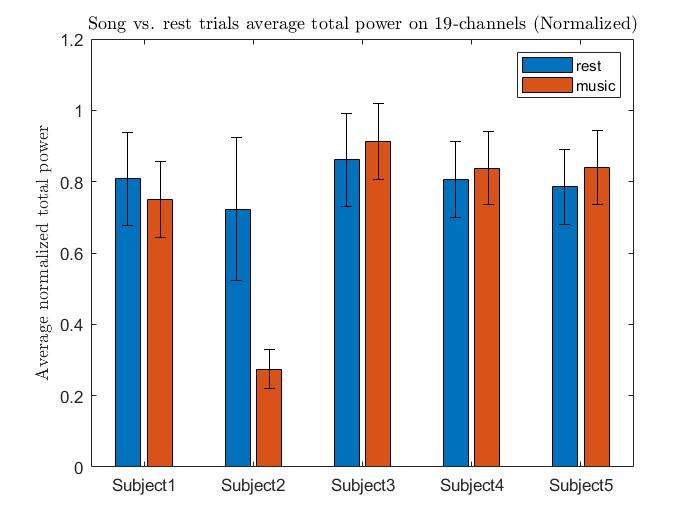
\includegraphics[width=0.9\linewidth]{SongVsRest.jpg}
 	\caption{Comparison between music and rest trials. Blue bars indicate the average power of rest trials for each subject. Red bars indicate the average power of song trials. The error bars are the standard deviation values. The data are normalized to their maximum values.}
  	\label{fig:SongVsRest}
\end{figure}

The comparison has been done between the average power of all five rest and song trials. The average power is evaluated by averaging over all 19 channels. Because of different conditions during data acquisitions (e.g. subjects' hair, scalp, and electrode impedance differences) scale of evaluated powers are different for each subject. Therefore evaluated powers are normalized by dividing to their maximum value so that we can compare them all together. As Figure \ref{fig:SongVsRest} indicates, the average power in song trials is less than the rest of the trials in subjects 1 and 2, while it has been increased for subjects 3, 4, and 5. Furthermore, this difference between subjects remains a question. It could be because of the nature of the subjectiveness of the task. \\

\begin{figure}[!htbp]
  \centering
  \begin{subfigure}[b]{0.4\linewidth}
    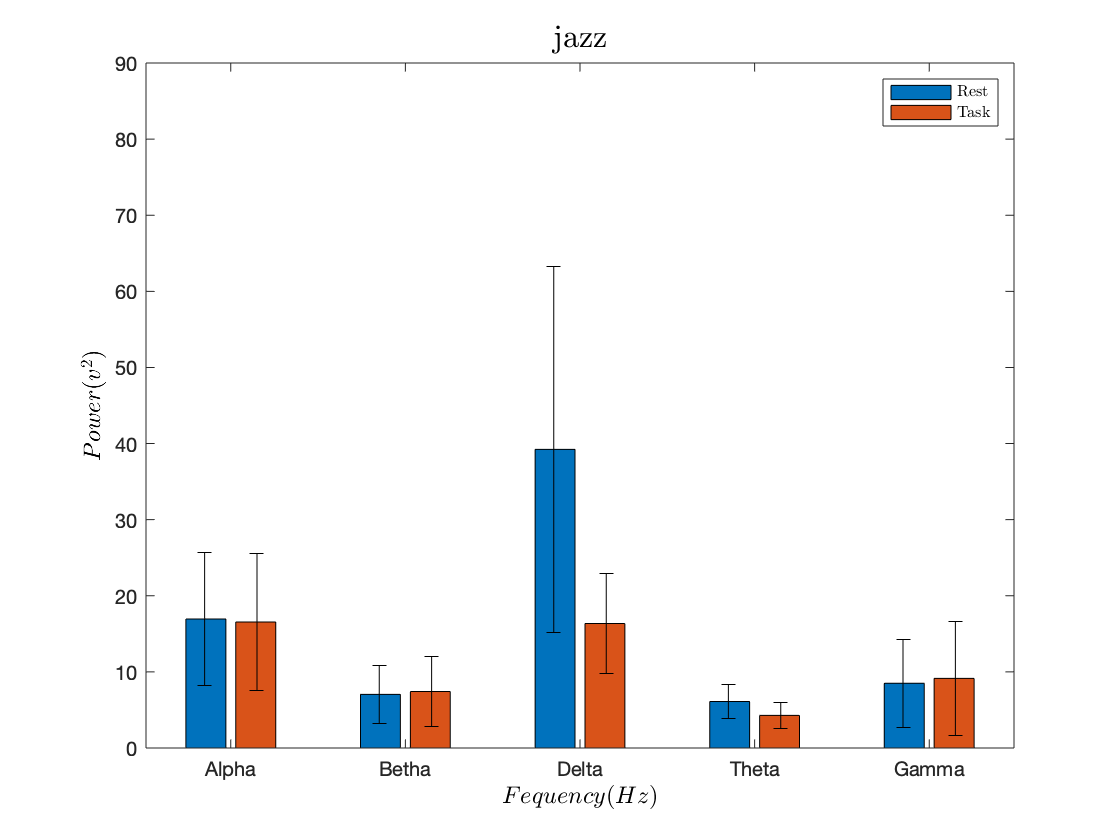
\includegraphics[width=\linewidth]{figures/jazz_RT.png}
  \end{subfigure}
  \begin{subfigure}[b]{0.4\linewidth}
    \includegraphics[width=\linewidth]{figures/rock_RT.png}
  \end{subfigure}
   \begin{subfigure}[b]{0.4\linewidth}
    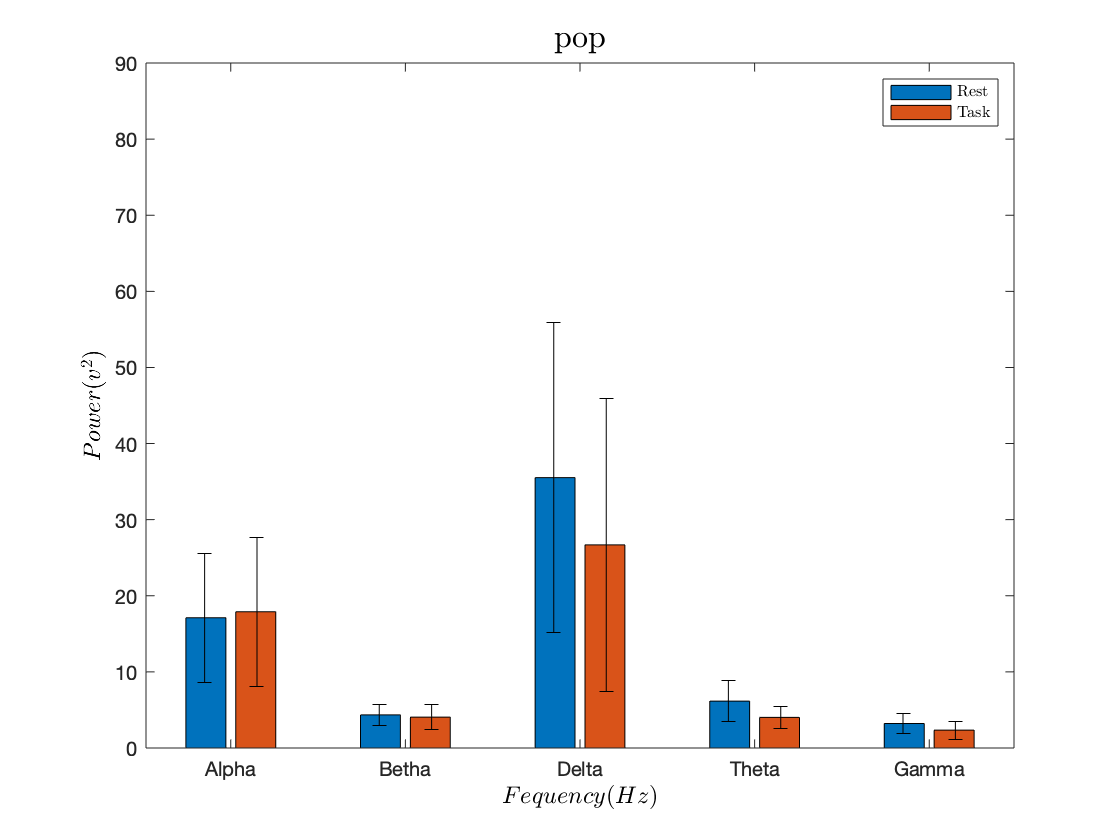
\includegraphics[width=\linewidth]{figures/pop_RT.png}
  \end{subfigure}
   \begin{subfigure}[b]{0.4\linewidth}
    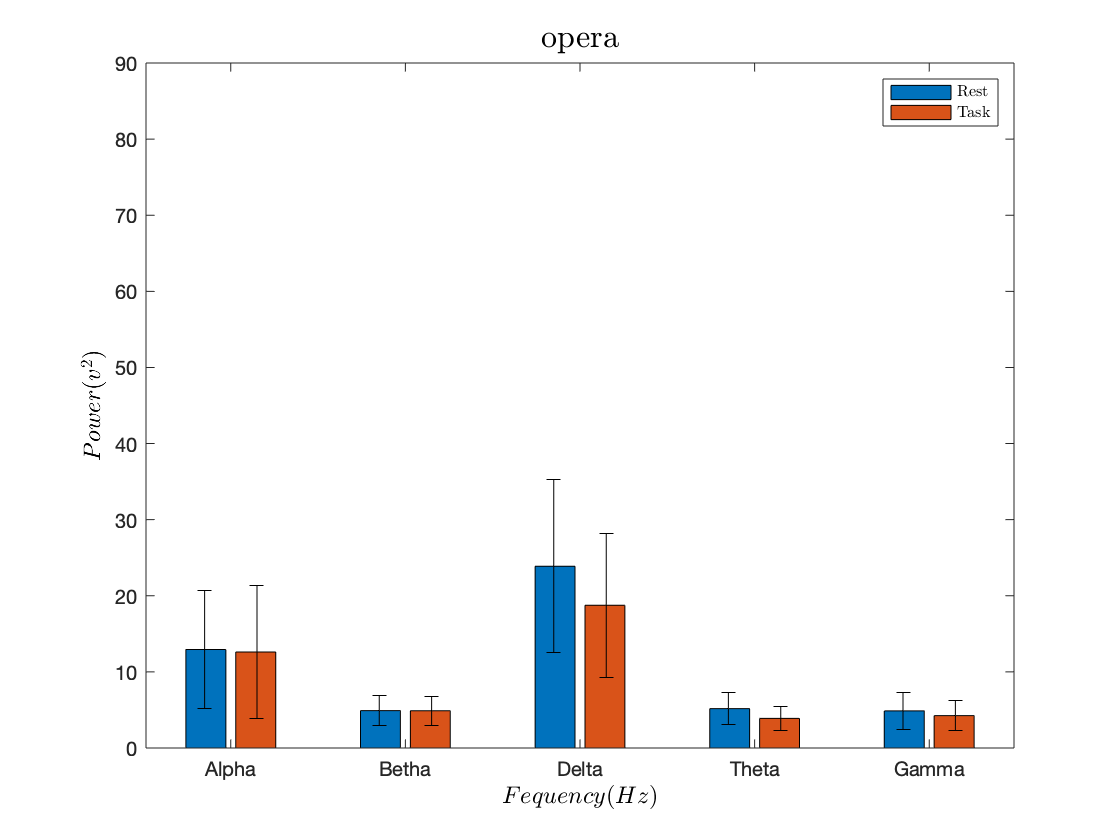
\includegraphics[width=\linewidth]{figures/opera_RT.png}
  \end{subfigure}
   \begin{subfigure}[b]{0.4\linewidth}
    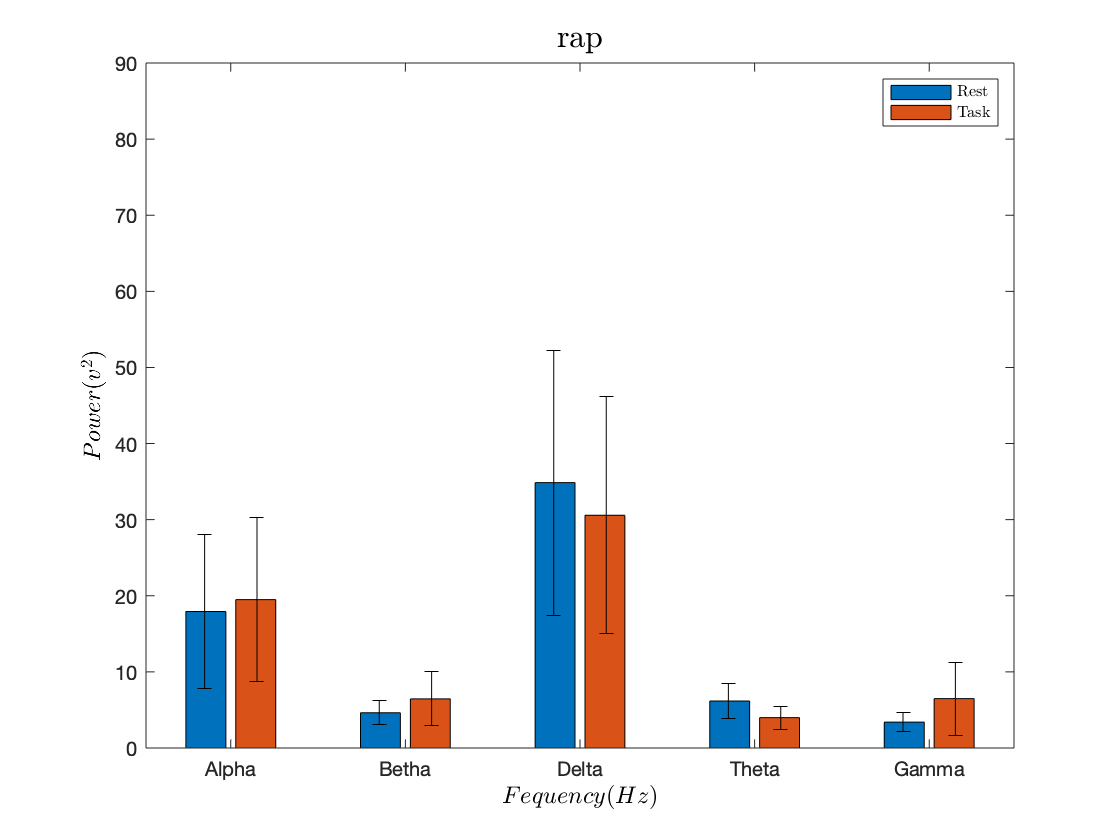
\includegraphics[width=\linewidth]{figures/rap_RT.png}
    
  \end{subfigure}
  \caption{Blue bars denote the average of each subject’s frequency band power at rest while orange ones show it during the music.
The length of the black lines indicates the standard deviation (STD) of the subject’s frequency band powers.
}
  \label{fig:GenresRT}
\end{figure}

Bands power to each specific genre. For each music genre, the percentage of subjects showing an increment in average power of each frequency band is indicated using the bar graph. The averaging is done over all 19 channels (Figure \ref{fig:subplot6reg} (top)). e.g. 60\% of subjects' beta band power has increased when listening to jazz music. The same analysis process has been done for six brain regions. \cite{kabuto1993} Frontal right (FP2, F4), frontal left (FP1, F3), parietal right (F4, P4), parietal left (F3, P3), occipital right (P4, O2), and occipital left (P3, O1). (Figure \ref{fig:subplot6reg} 2nd, 3rd and 4th rows). According to Figure \ref{fig:subplot6reg}, Jazz music has affected alpha band power the least. (20\% in all regions and 40\% in FR region). 40\% of subjects have shown an increase in alpha band power while listening to pop music in all the regions. Also, the alpha band power of 60\% of subjects (which is greater than half) has increased in rap music trials. The more detailed information resulted from Figure \ref{fig:subplot6reg} is indicated in Table \ref{table:6reg}.\\ 

\begin{table}[h!]%[tbhp]
\centering
\caption{6 regions percentage of power increment}
\label{table:6reg}
\begin{tabular}{lrrrrrr}
\textbf{Total} & Alpha & Beta & Gamma & Delta & Theta \\
\midrule
Jazz & - & 60\% & - & 60\% & - \\
Rock & - & 60\% & 60\% & - & - \\
Rap & - & - & - & 60\% & 60\% \\
\bottomrule
\end{tabular}

\begin{tabular}{lrrrrrr}
\textbf{FR} & Alpha & Beta & Gamma & Delta & Theta \\
\midrule
Jazz & - & - & 60\% & - & - \\
Pop & - & 60\% & - & - & - \\
Rock & - & - & - & - & 60\% \\
Rap & 60\% & - & - & 60\% & 60\% \\
\bottomrule
\end{tabular}

\begin{tabular}{lrrrrrr}
\textbf{FL} & Alpha & Beta & Gamma & Delta & Theta \\
\midrule
Jazz & - & - & - & 60\% & 60\% \\
Rock & - & 60\% & - & - & 60\% \\
Rap & 60\% & - & - & - & 60\% \\
\bottomrule
\end{tabular}

\begin{tabular}{lrrrrrr}
\textbf{PR} & Alpha & Beta & Gamma & Delta & Theta \\
\midrule
Jazz & - & - & - & 60\% & - \\
Rock & - & 60\% & - & - & 60\% \\
Rap & 60\% & 60\% & - & - & 60\% \\
\bottomrule
\end{tabular}

\begin{tabular}{lrrrrrr}
\textbf{PL} & Alpha & Beta & Gamma & Delta & Theta \\
\midrule
Jazz & - & 80\% & - & - & 60\% \\
Rap & 60\% & - & - & - & - \\
\bottomrule
\end{tabular}

\begin{tabular}{lrrrrrr}
\textbf{OR} & Alpha & Beta & Gamma & Delta & Theta \\
\midrule
Jazz & - & 60\% & - & 60\% & - \\
Rap & 60\% & - & - & - & 60\% \\
\bottomrule
\end{tabular}

\begin{tabular}{lrrrrrr}
\textbf{OL} & Alpha & Beta & Gamma & Delta & Theta \\
\midrule
Rap & 60\% & 60\% & - & - & - \\
\bottomrule
\end{tabular}

\addtabletext{only increments of more than 50\% are mentioned}
\end{table}

As can be seen in Figure \ref{fig:GenresRT}, the power of delta and theta bands have been reduced in all of the genres. According to Table \ref{table:BrainWaves}, delta and theta bands are related to dreamless sleep and drowsiness states; therefore, they should be decreased during the auditory stimuli which require concentration. 
In this part, the impact of each genre on the power of frequency bands have been studied.
 During playing the rap song, the power of gamma and betta bands have been raised while in the other songs they haven’t been changed notably. It is noteworthy that because of the small sample size, the STD of some of the frequency bands is high, so it may cause uncertainty in the obtained results. \\


According to the aim of this study, we analyze the relationship between the difference of frequency band powers (before and after playing song) and changes in subject’s mental states for each genre (it is obtained from a questionnaire filled out by subjects) To validate the above analysis, the absolute value of correlation must be over 0.7 to be selected as a significant relation.\cite{Sedghizadeh2020}. Results are written down in Table \ref{table:result1} and are shown in Figure \ref{fig:Corrplot}.\\

Percentage of Subjects with Increment or decrement in feelings is reported in Table \ref{table:POIOD}.\\

\begin{table}[ht]
\caption{Brain Waves and Mental States \cite{Abhang2016}}
\label{table:BrainWaves}
\centering
\begin{tabular}{p{0.2\linewidth} p{0.2\linewidth} p{0.4\linewidth}}
Brain Wave & Frequency Interval & Mental State \\  [0.5ex]
\hline
Delta  & 0.5 - 3 Hz & Produced in deep, dreamless sleep\\
Thteta & 4 - 7 Hz  & Drowsiness, inattention, deep meditation\\
Alpha & 8 - 12 Hz  & General relaxation and meditation \\
Beta Low& 12 - 15 Hz  &   Relaxed concentration \\
Beta Midrange& 15 - 20 Hz  &   Foucused attention \\
Beta High& 20 - 30 Hz  &   Anxiety \\
Gamma& $>$ 30 Hz  &   hypnotic states, expanded consciousness \\
[1ex]
\hline
\end{tabular}
\end{table}

\begin{figure}[!htbp]
  \centering
  \begin{subfigure}[b]{0.4\linewidth}
    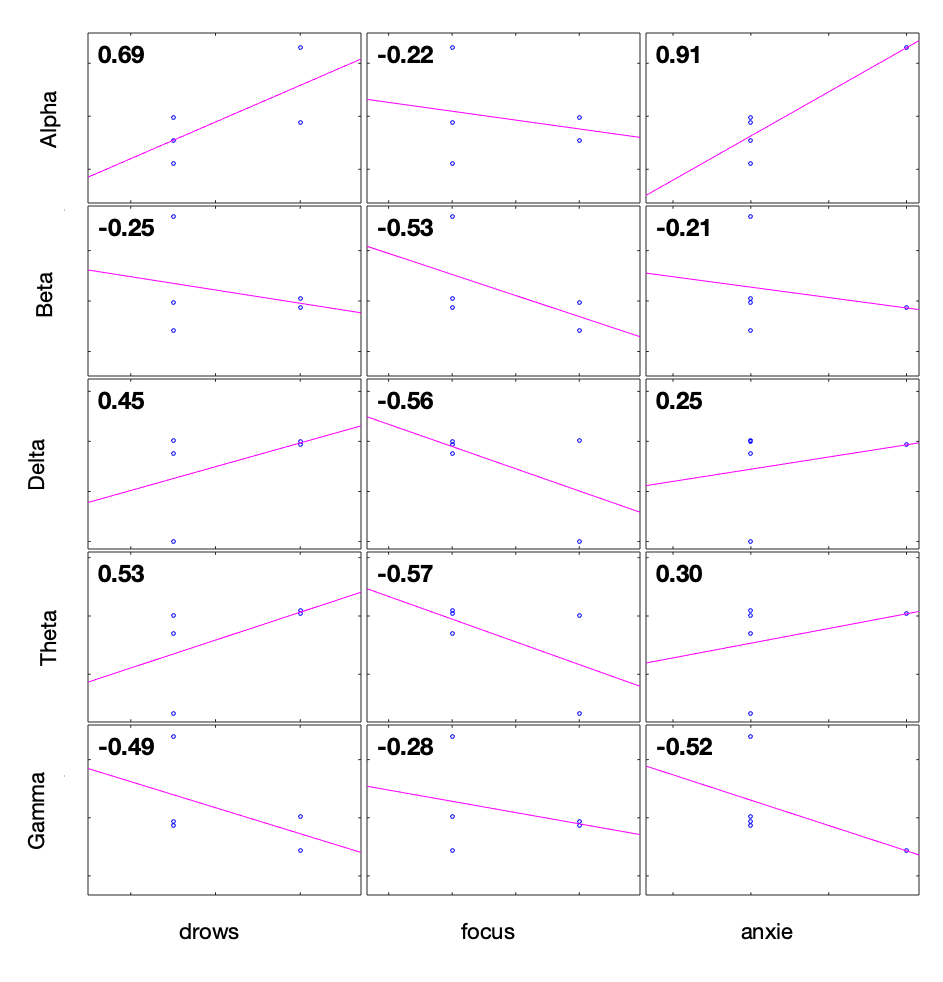
\includegraphics[width=\linewidth]{figures/jazz_corrplot.png}
    \caption{Jazz CorrPlot}
  \end{subfigure}
  \begin{subfigure}[b]{0.4\linewidth}
    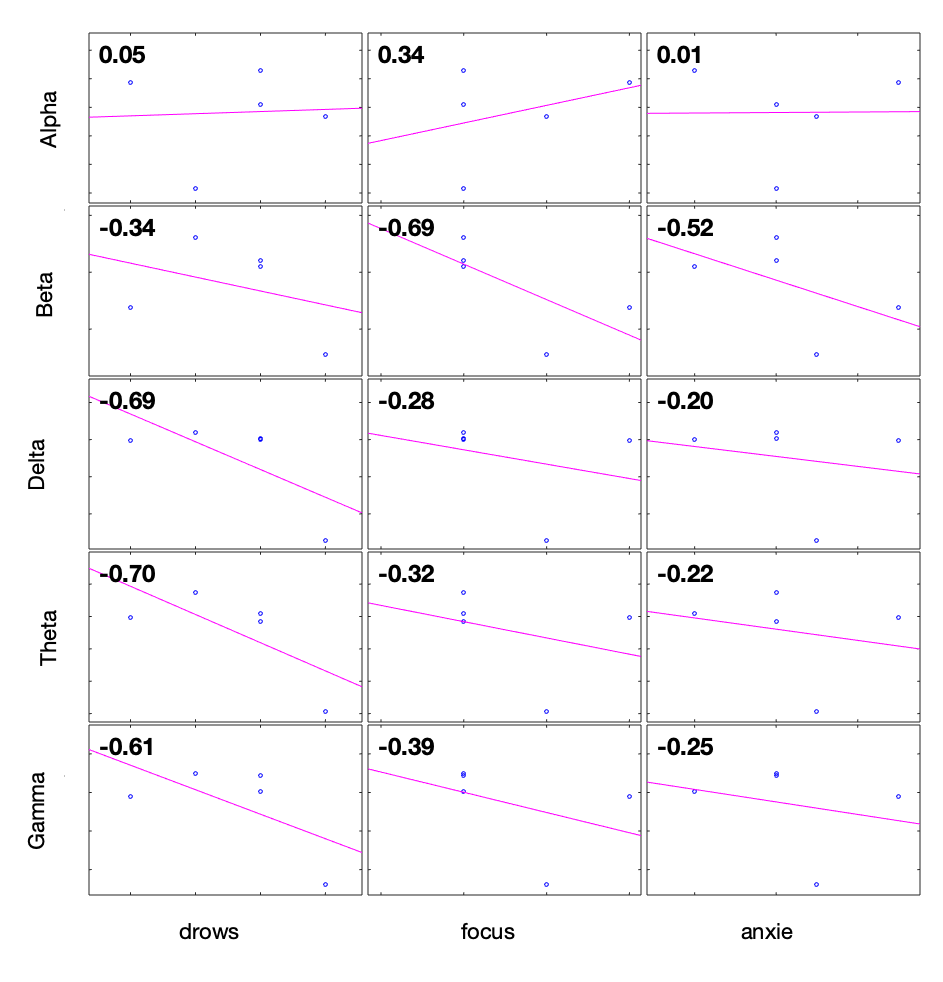
\includegraphics[width=\linewidth]{figures/rock_corrplot.png}
    \caption{Rock CorrPlot}
  \end{subfigure}
   \begin{subfigure}[b]{0.4\linewidth}
    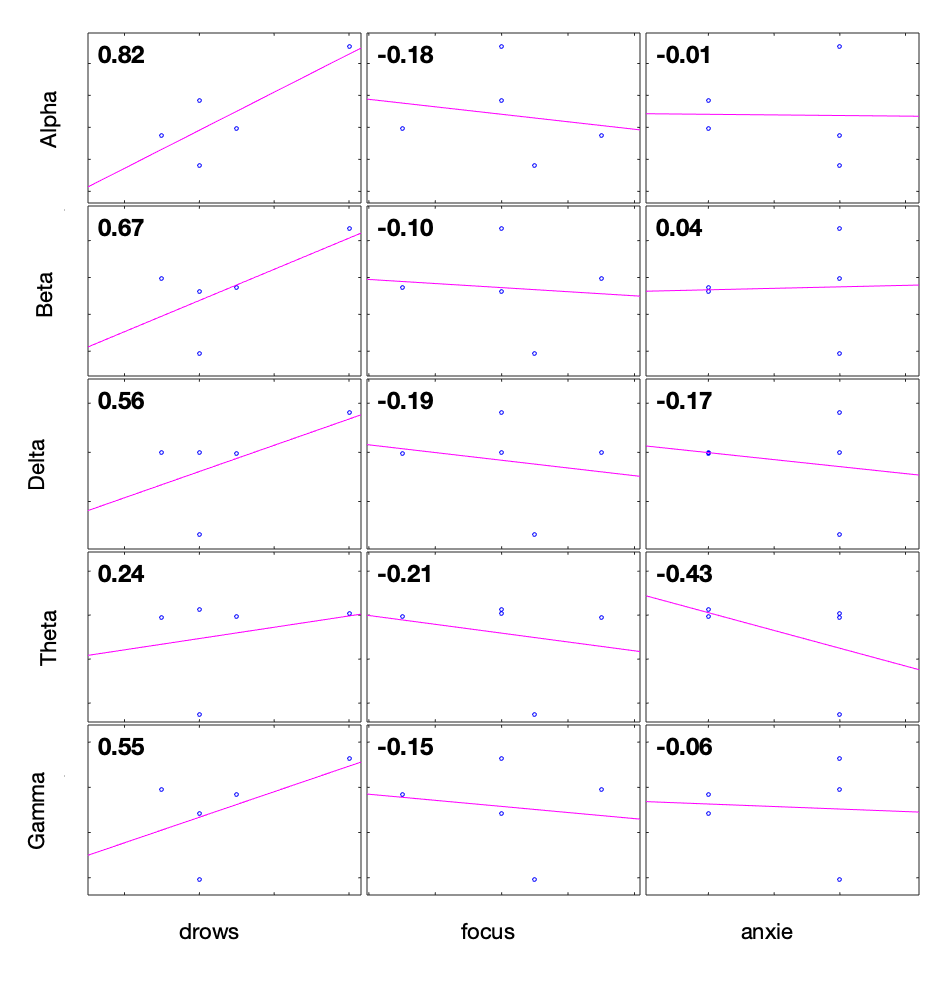
\includegraphics[width=\linewidth]{figures/pop_corrplot.png}
    \caption{Pop CorrPlot}
  \end{subfigure}
   \begin{subfigure}[b]{0.4\linewidth}
    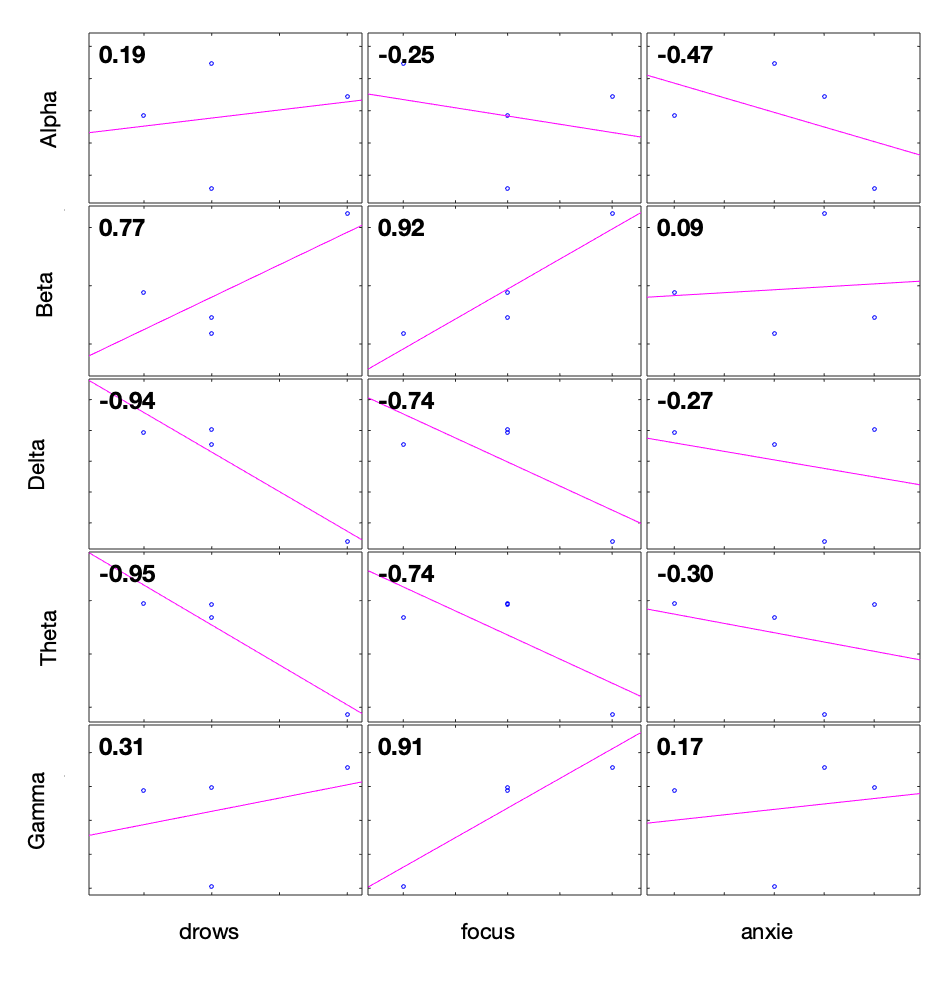
\includegraphics[width=\linewidth]{figures/opera_corrplot.png}
    \caption{Opera CorrPlot}
  \end{subfigure}
   \begin{subfigure}[b]{0.4\linewidth}
    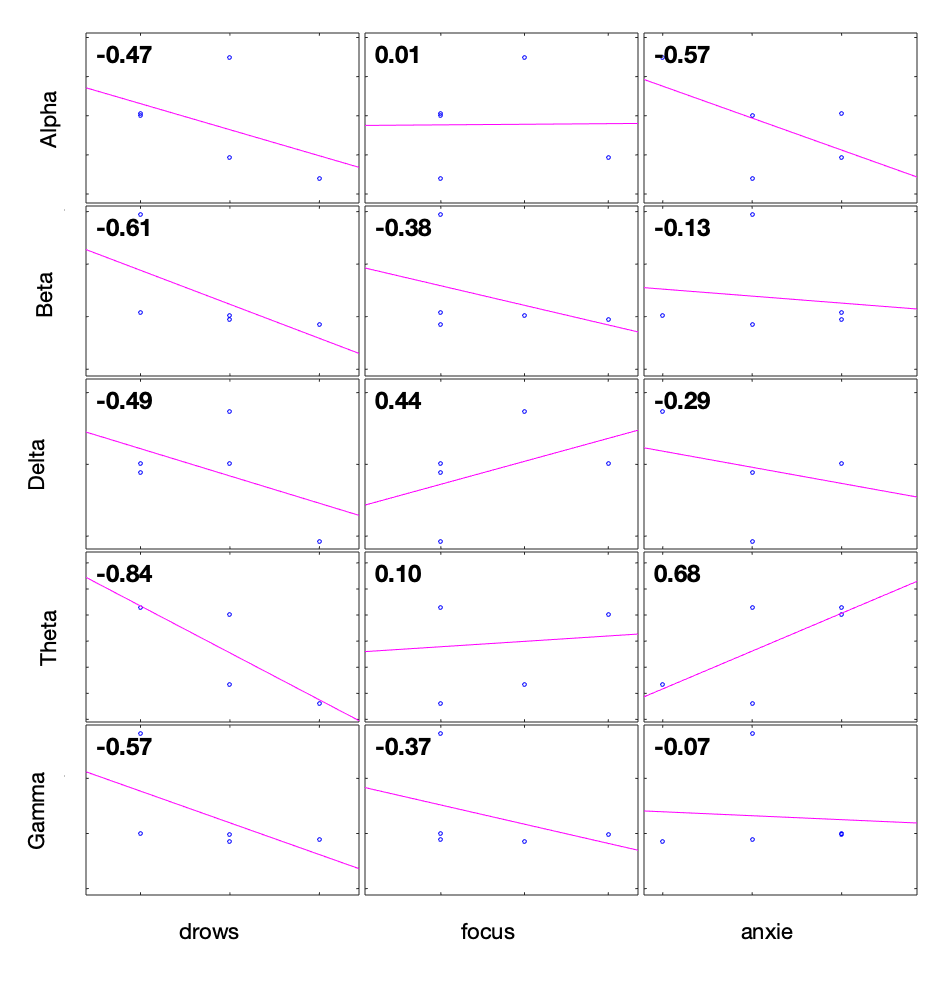
\includegraphics[width=\linewidth]{figures/rap_corrplot.png}
    \caption{Rap CorrPlot}
  \end{subfigure}
  \caption{The pink lines plotted in each window are linear regression of two variables and points in each window indicate the locations of variables for each subject. Xaxis labels correspond to the changes of mental states asked in the questionnaire(without unit). The number in each window shows the correlation between two variables.
}
  \label{fig:Corrplot}
\end{figure}

\begin{table}[ht]
\raggedleft
  \caption{Relation between Song Genres and Mental States}
\label{table:result1}
\begin{tabular}{p{0.1\linewidth}|p{0.8\linewidth}}
  \textbf{Genre} & \textbf{Effect} \\
\hline
Jazz& Alpha is positively correlated to anxiety feeling.\\
Opera&In contrast of positive link between beta to drowsiness and focus, delta and theta are inversely correlated to drowsiness and focus, Also gamma is directly linked to focus.\\
Pop &Alpha is positively associated with drowsiness.\\
Rap &Theta has a reverse correlation to drowsiness feeling.\\
Rock &Theta is negatively associated with drowsiness.\\
\end{tabular}
\end{table}


\begin{table}
\centering
\caption{Percentage of Subjects with Increment or decrement in feelings  (obtained from Questionnaire) }
\label{table:POIOD}
  \begin{tabular}{c | c c | c c | c c}
        \multirow{2}{*}{Genres} &
      \multicolumn{2}{c}{Drowsy} &
      \multicolumn{2}{c}{Focused} &
      \multicolumn{2}{c}{Anxious} \\
    & Inc & Dec & Inc& Dec & Inc & Dec \\
    \hline
    Pop & 0\% & 100\% & 0\% & 100\% & 0\% & 60\% \\
        Rock & 20\% & 60\% & 20\% & 60\% & 20\% & 60\% \\
        Opera & 40\% & 60\% & 40\% & 60\% & 40\% & 40\% \\
        Jazz & 0\% & 100\% & 0\% & 100\% & 0\% & 60\% \\
        Rap & 40\% & 60\% & 40\% & 60\% & 40\% & 40\% \\
      \end{tabular}
\end{table}





\begin{figure*}[h!]
	\centering
	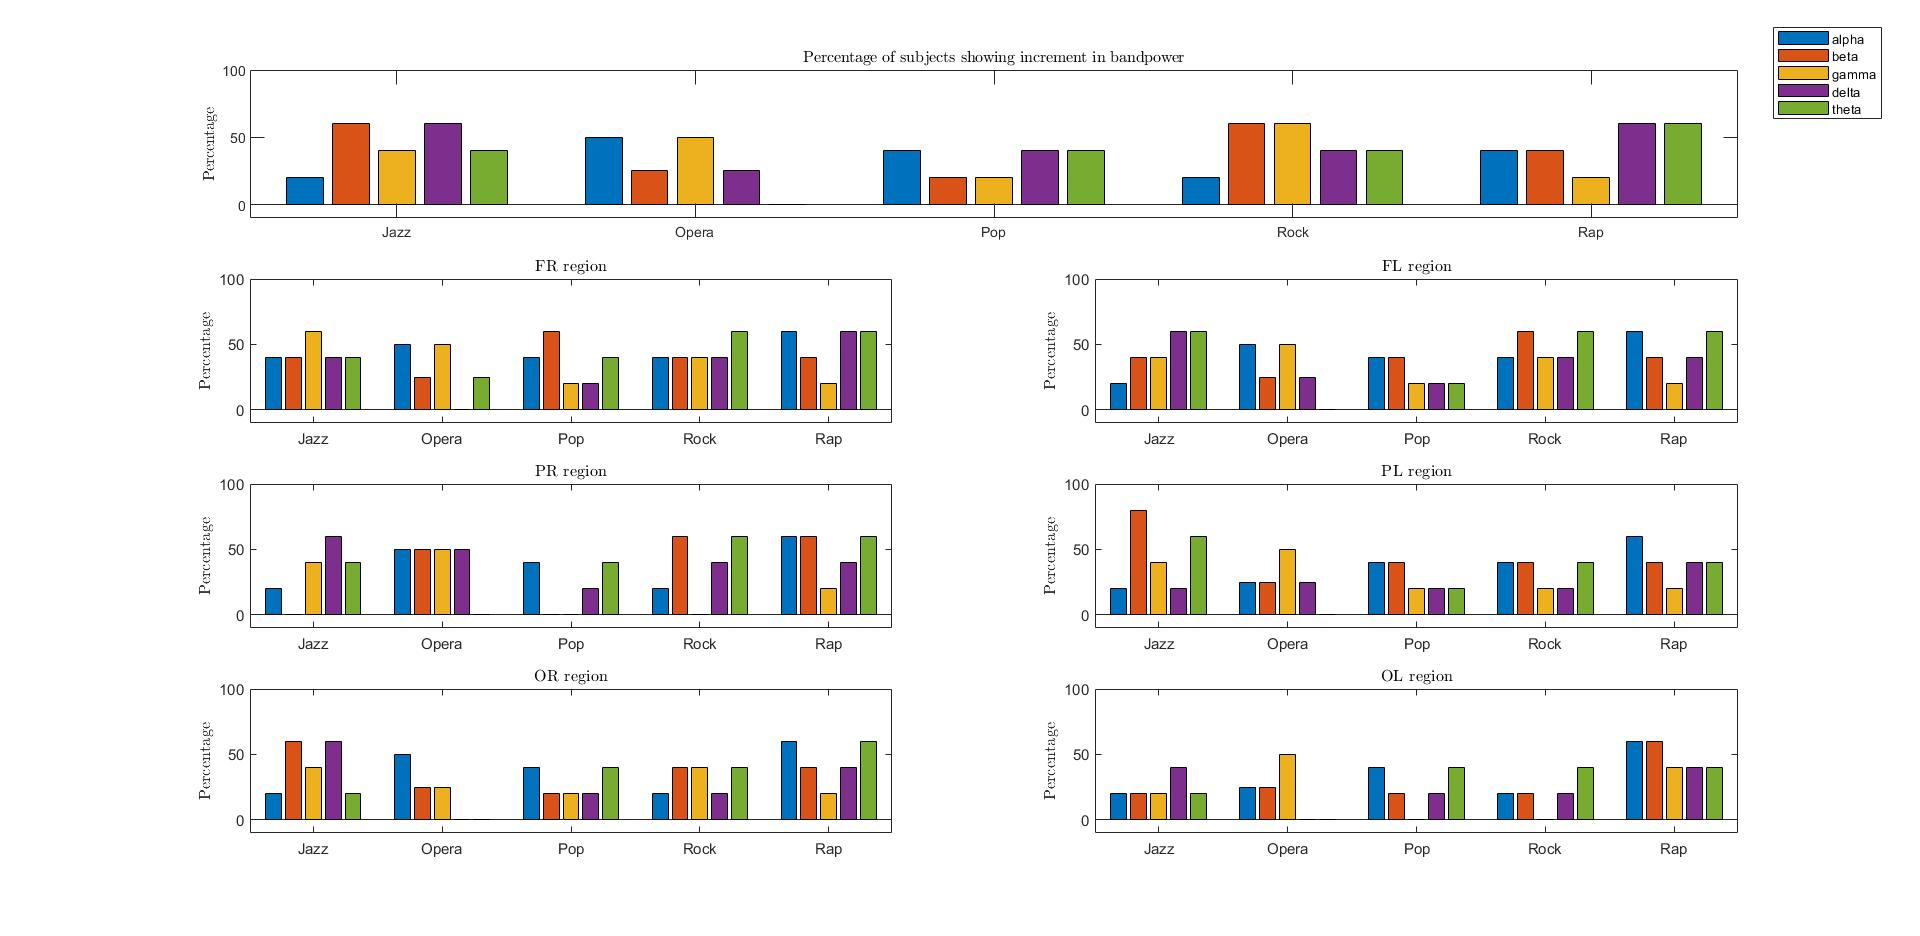
\includegraphics[width=0.8\linewidth]{subplot6reg.jpg}
 	\caption{Percentage of subjects that showed an increment in each band power during each music genre trials. Top) the band powers are averaged over all 19 channels. The second row left) average over the FR region (FP2, F4). Second row right) average over the FL region (FP1, F3). The third row left) average over PR region (F4, P4). Third row right) average over PL region (P3, F3). The fourth row left) average over OR region (P4, O2). Fourth row right) average over OL region (P3, O1).}
  	\label{fig:subplot6reg}
\end{figure*}

\section*{Discussion}
The relation between frequency bands' power and music genres was investigated as the main result of this study. Reduction of delta and theta bands power in all of the genres was observed, moreover rap songs increase the power of gamma and beta bands while other genres don’t have a remarkable effect on frequency bands power. As a sub result of this study, the relation between mental states and frequency bands power in each genre are displayed in Figure \ref{fig:Corrplot}.\\

In this study, In harmony with previous researches \cite{kabuto1993,Wagner1975}, frequency bands power, and mental states are used as two unknown variables which the relation between them is inquired.  In contrary to Related Articles \cite{kabuto1993,Verrusio2015,Wagner1975} that the effect of a specific pleasant song on mental states was discussed, in this paper the effects of five different genres(pop, rock, jazz, rap, and opera) are scrutinized. in 1993, Michinori KABUTO et al. declared that theta and beta bands power have a reverse correlation to relaxed feeling while beta band power is positively correlated to sharp and active feeling, also our results about music effect on the relation between mental states (which are different from the mentioned article) and power of frequency bands are shown in Figure \ref{fig:Corrplot}.\\

The results of this study can be a suitable guide for further studies on the relation between music and mental states, especially in music therapy. Also, in the future, these results could be a good guide for research on the frequency content of songs and their effects on human emotions, so that by opting for the most appropriate music with a particular frequency content as a stimulus, certain bands of the brain became activated, each of which can induce a special feeling in humans. \\ 




%\begin{figure}%[tbhp]
%\centering
%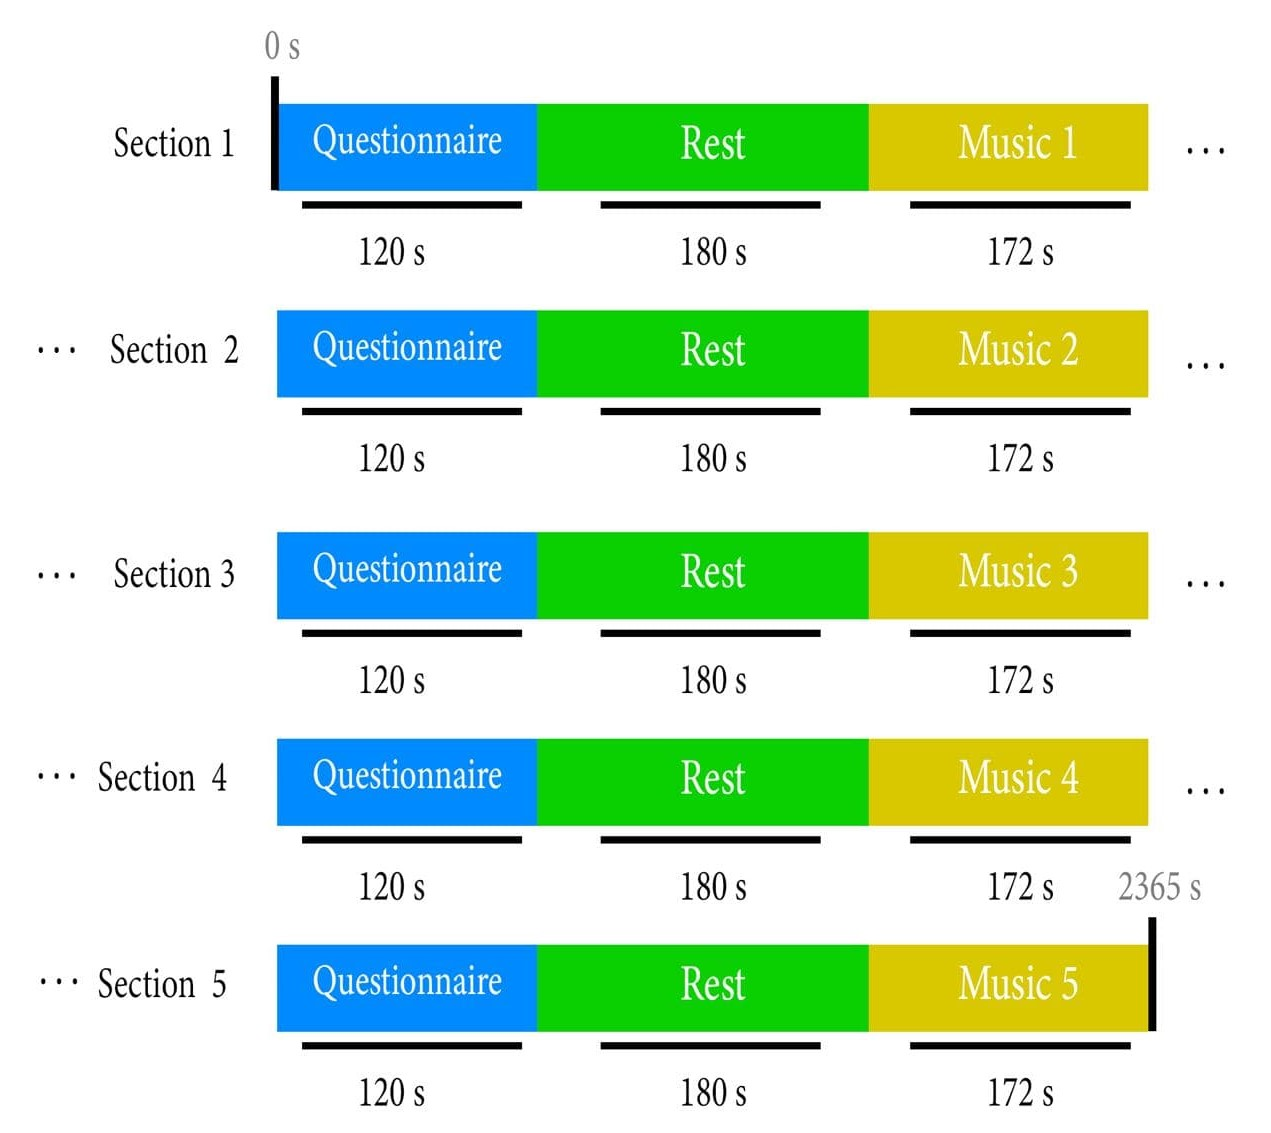
\includegraphics[width=.8\linewidth]{Timeline}
%\caption{Placeholder image of a frog with a long example caption to show justification setting.}
%\label{fig:frog}
%\end{figure}

%\begin{SCfigure*}[\sidecaptionrelwidth][t]
%\centering
%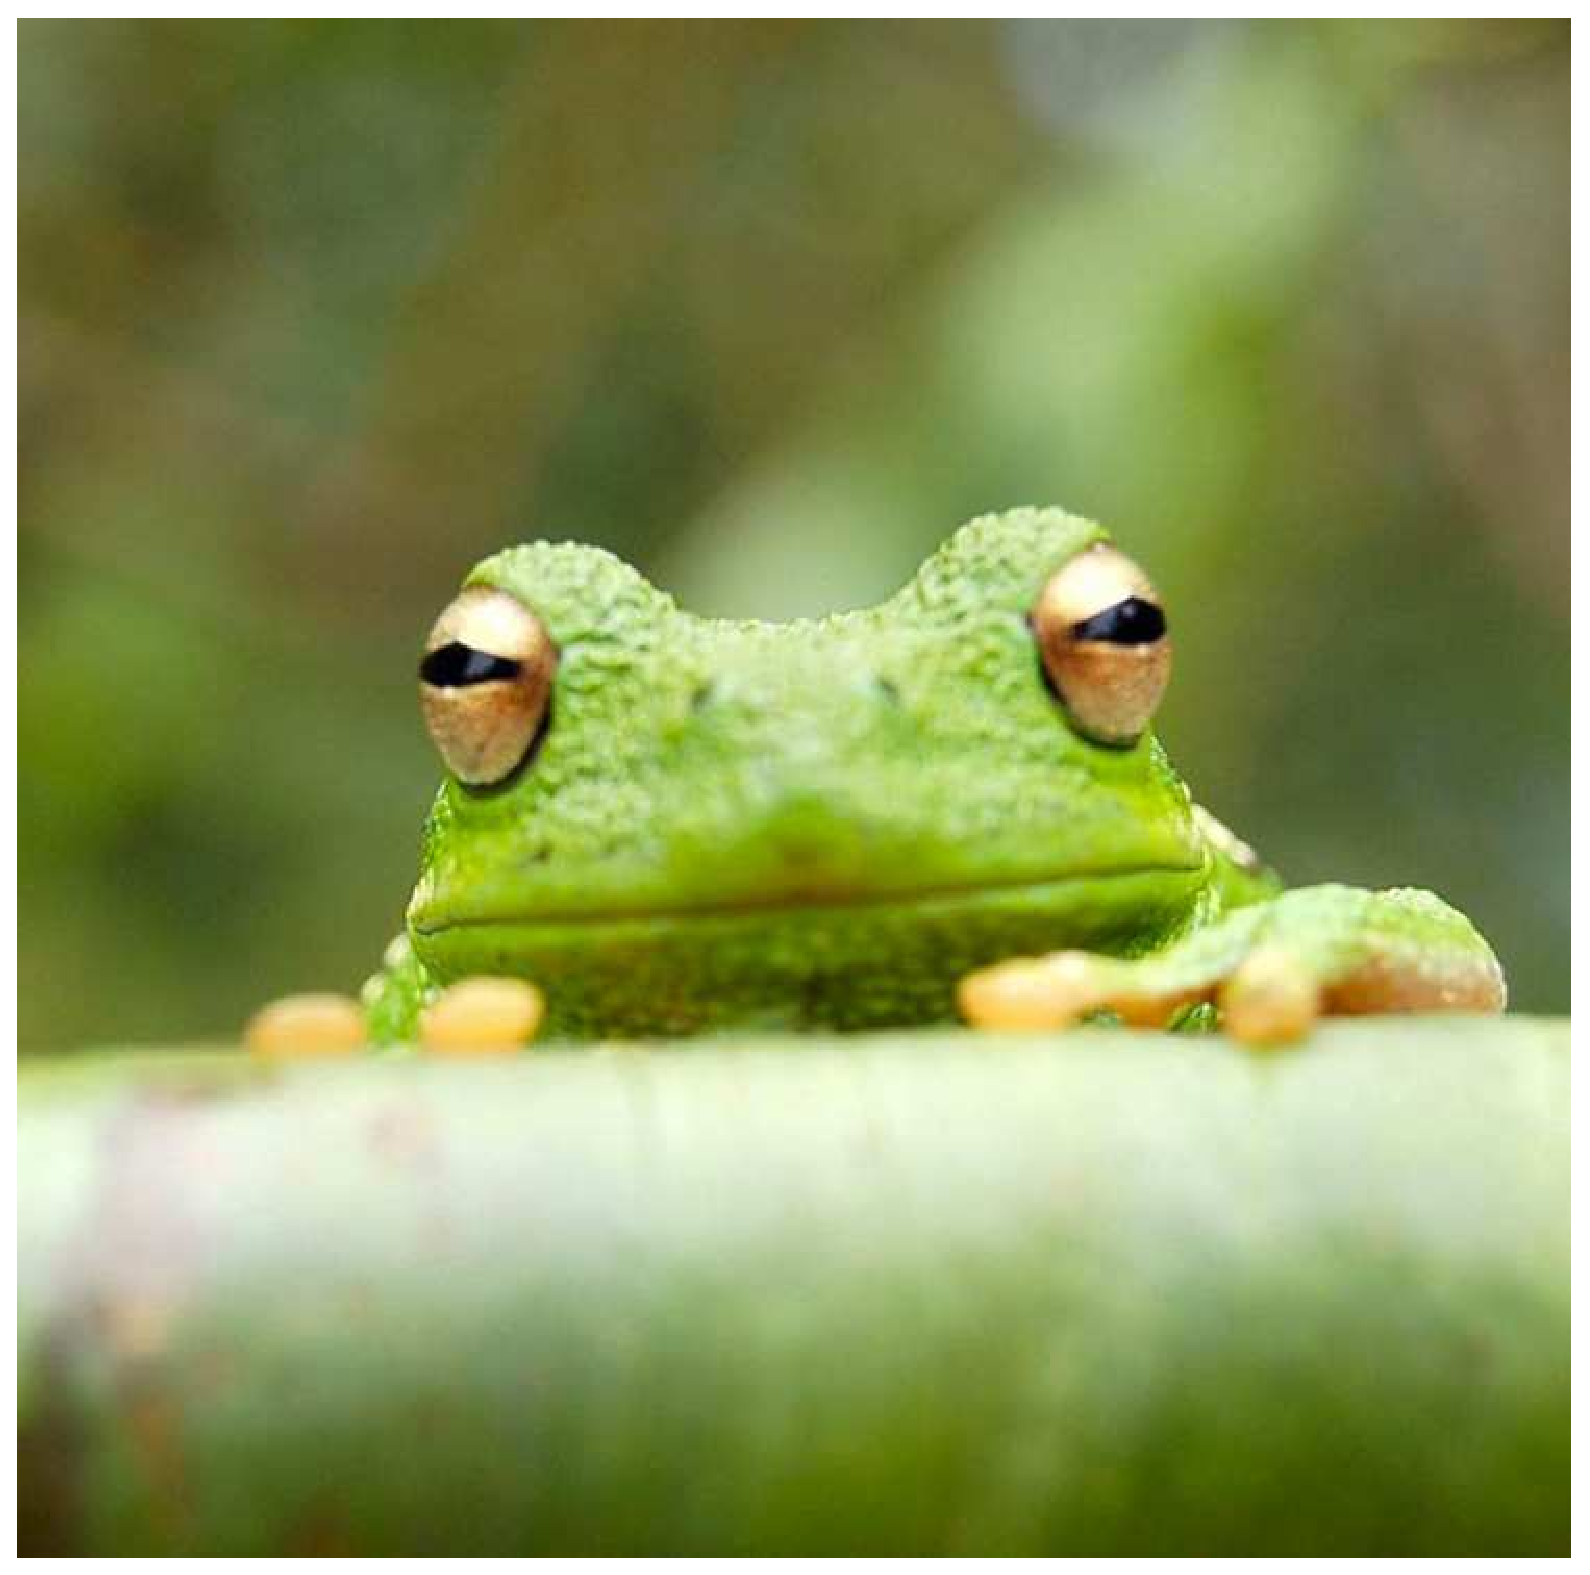
\includegraphics[width=11.4cm,height=11.4cm]{frog}
%\caption{This caption would be placed at the side of the figure, rather than below it.}\label{fig:side}
%\end{SCfigure*}

\section*{Materials and Methods}

The subjects were 5 healthy males and females with normal hearing and an average of 20 years old (20-21). Detailed information about subjects are shown in Table \ref{table:SubInf}.\\
\begin{table}[h!]%[tbhp]
\centering
\caption{Subjects Informaton}
\label{table:SubInf}
\begin{tabular}{lrrrr}
 & Sex & Age & Lesions & Name\\
\midrule
Subject 1 & M & 20 & - & Ali Ghavampour\\
Subject 2 & F & 20 & - & Maryam Maghsoudi\\
Subject 3 & M & 20 & - & Arsalan Firoozi\\
Subject 4 & M & 21 & - & Alireza Tabrizi\\
Subject 5 & F & 20 & - &Yasamin Medghalchi\\
\bottomrule
\end{tabular}
\end{table}

There is a 15 minutes interval before the experiment begins to inform the subjects about the task procedure and filling out the questionnaire before the first song to inquire about their mental states (Table \ref{table:Ques}). The task consists of 5 sections including two trials, A trial of 180 seconds rest, a trial of 172 seconds of music stimuli, and a 2-minute interval for answering the questionnaire after each song (a total of 10 trials without including questionnaire time). Timeline is displayed in Figure \ref{fig:Timeline} a. \\


\begin{figure}[h!]
  \centering
  \begin{subfigure}[b]{0.7\linewidth}
    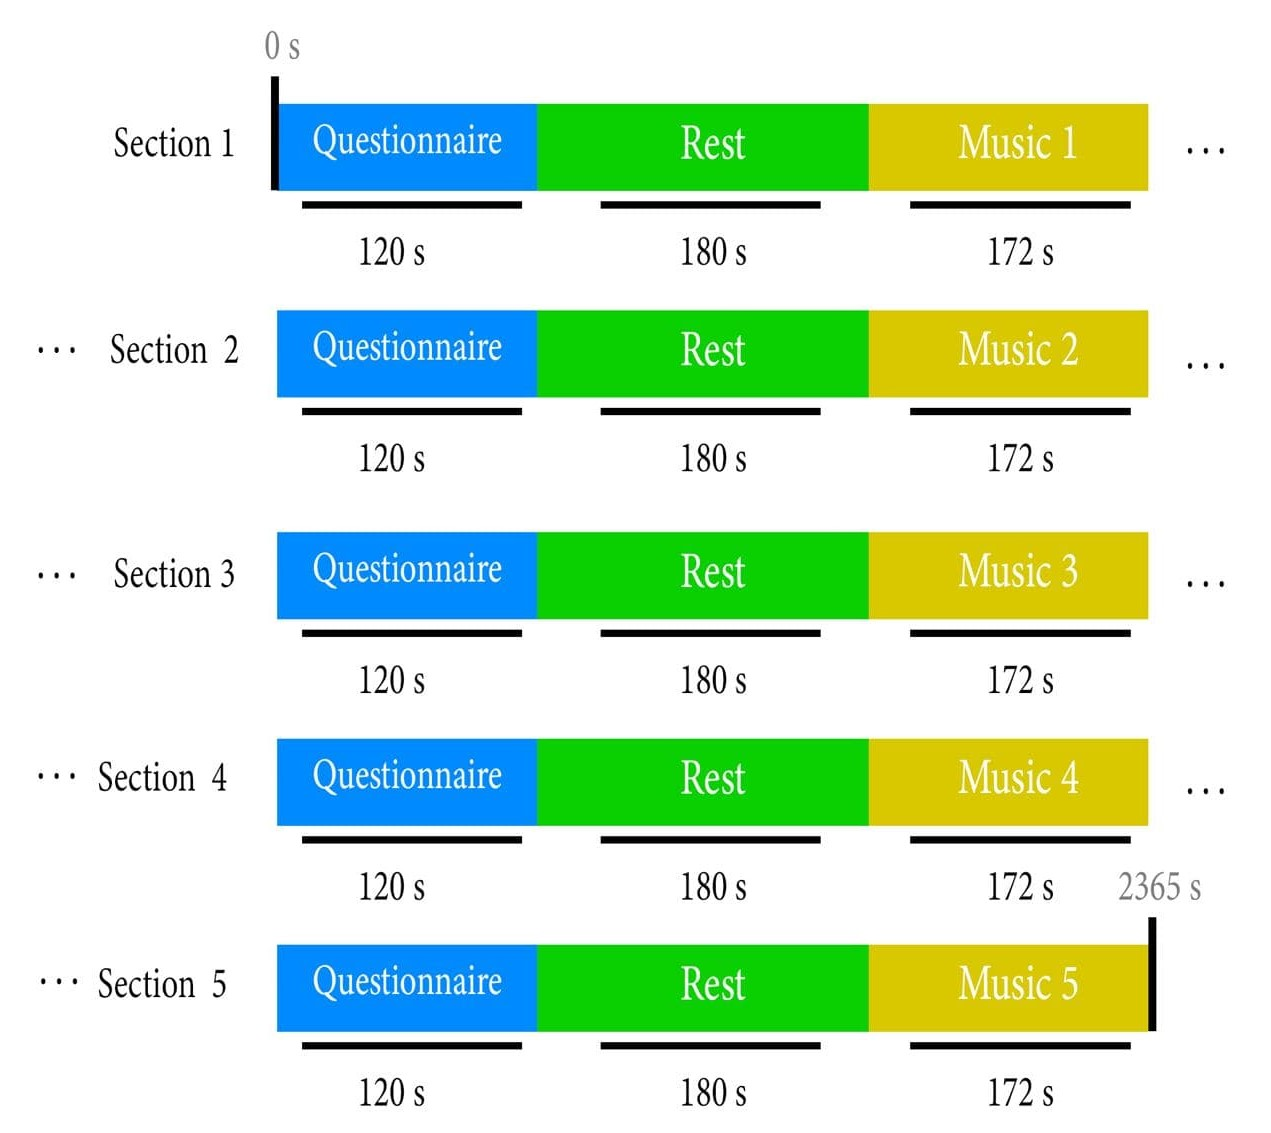
\includegraphics[width=\linewidth]{Timeline.jpg}
    \caption{}
  \end{subfigure}
  \begin{subfigure}[b]{0.7\linewidth}
    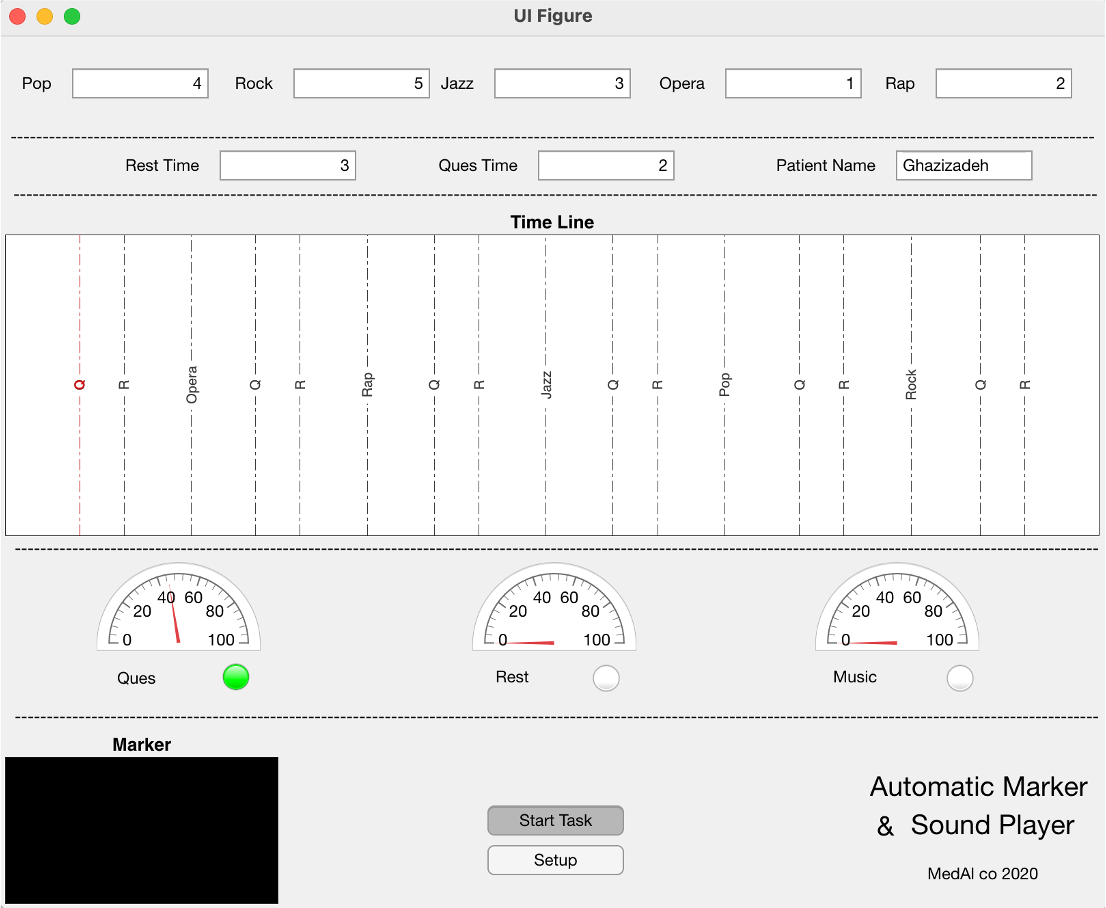
\includegraphics[width=\linewidth]{GUI.png}
    \caption{}
  \end{subfigure}
  \caption{(a) is a diagram for better understanding of task. (b) is a MATLAB GUI developed by us to produce triggers for EEG data.}
  \label{fig:Timeline}
\end{figure}

One of the most popular songs of each genre (Pop, Rock, Jazz, Opera, Rap) was selected from Apple iTunes and was played for the subjects in each section (Table \ref{table:Songs}). The order of playing songs was identical for 3 subjects, other subjects listened to a randomly different order to take the song order dependency effect into account (Though no dependence has been seen). EEG was recorded by the bipolar method using NrSign 64 channel EEG device (Negar Andishegan co.) and in standard 10-20 system. The impedance of electrodes was held under $15k\Omega$ during data acquisition. Subjects were sitting on a chair with open eyes in front of a white wall in a dark room. Each song was played through a speaker placed one meter behind the subject\textquotesingle s chair. \\


Makato’s pipeline \cite{Makato} and EEGLAB MATLAB software \cite{eeglab} were used for preprocessing. First, data were downsampled to 200Hz (sampling rate is 500Hz in NrSign EEG device) and bad parts were removed by inspection. A bandpass 0.5-70Hz and a 50Hz notch filter (default EEG device filter) was applied to the acquired signal by EEG device. To reduce noise, all channels were re-referenced to average. The bad components (e.g. mouth and eye movements) and artifacts of the signal were removed by Independent Component Analysis (ICA).


\begin{table}[tbhp]
\centering
\caption{Selected Songs}
\label{table:Songs}
\begin{tabular}{lrrr}
Genre & Song & Artist\\
\midrule
Rock & Shot In The Dark & AC/DC\\
Jazz & Sing Sing Sing & Benny Goodman\\
Opera & Marriage of Figaro Voi Che Sepate & Mozart\\
Pop & Swimming in The Stars & Britney Spears\\
Rap & Lose Yourslef & Eminem\\
\bottomrule
\end{tabular}
\end{table}

\begin{table}[tbhp]
\centering
\caption{Questionnaire}
\label{table:Ques}
\begin{tabular}{lrrr}
Question & Answer\\
\midrule
How much do you feel drowsy? & 1-10\\
How much do you feel focused? & 1-10\\
How much do you feel anxious? & 1-10\\
Have you heard this song before? & Yes-No\\
\bottomrule
\end{tabular}
\end{table}

It has been shown that band power can be used as a representative feature in musical and auditory tasks \cite{kabuto1993}. The average power of frequency bands (Alpha, Beta, Theta, Delta, Gamma) of each rest and song trials were evaluated. The power difference between rest and song trials was the focus of interest in this study. We calculated the average power over all channels and also on 6 regions of Figure \ref{fig:BrainRegions} just as Kabuto \cite{kabuto1993} did.\\

\begin{figure}[h!]
	\centering
	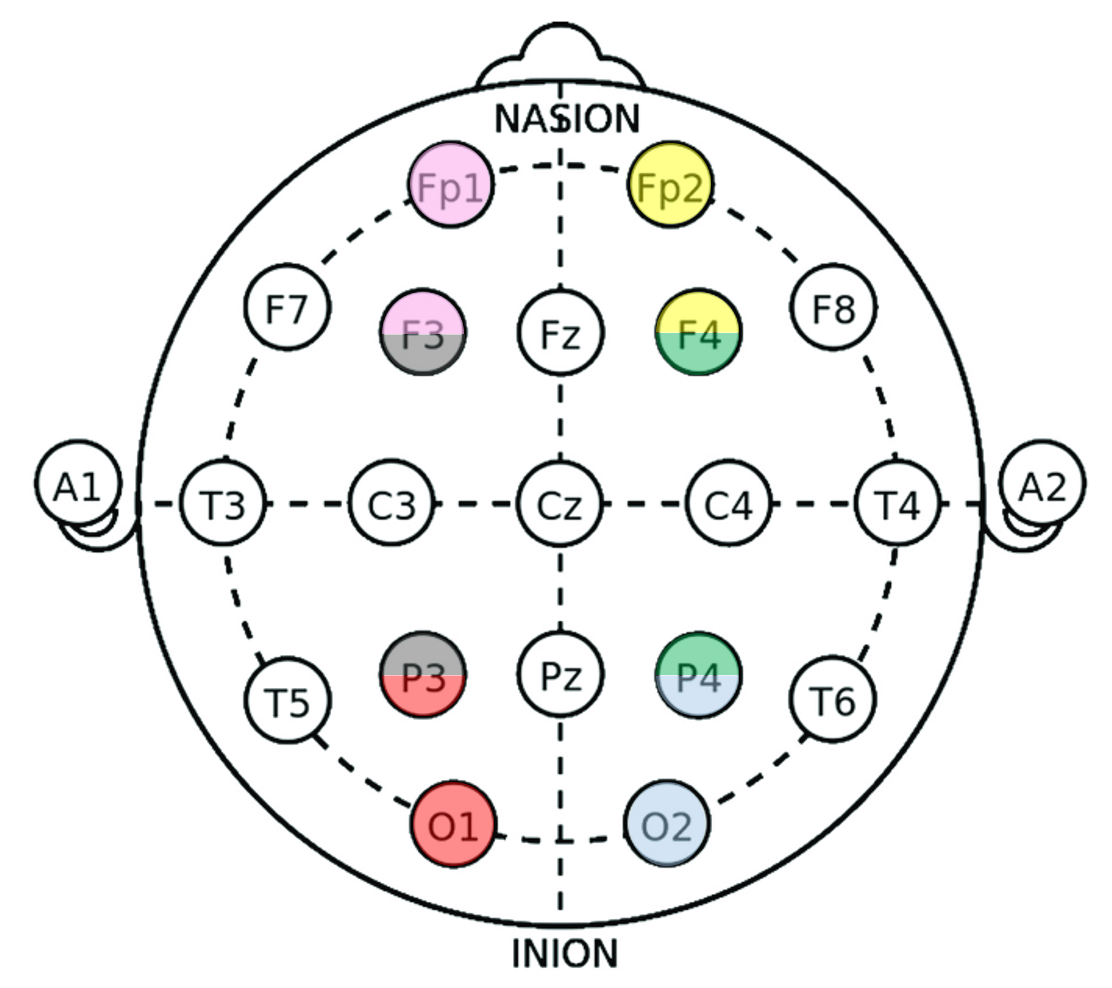
\includegraphics[width=0.8\linewidth]{BrainRegions.png}
 	\caption{Fronto Left: Pink, Fronto Right: Yellow, Parietal Left: Grey, Parietal Right: Green, Occipital Left: Red, Occipital Right: Blue}
  	\label{fig:BrainRegions}
\end{figure}

%\begin{figure*}[bt!]
%\begin{align*}
%(x+y)^3&=(x+y)(x+y)^2\\
   %    &=(x+y)(x^2+2xy+y^2) \numberthis \label{eqn:example} \\
      % &=x^3+3x^2y+3xy^3+x^3. 
%\end{align*}
%\end{figure*}

%\begin{table}%[tbhp]
%\centering
%\caption{Comparison of the fitted potential energy surfaces and ab initio benchmark electronic energy calculations}
%\begin{tabular}{lrrr}
%Species & CBS & CV & G3 \\
%\midrule
%1. Acetaldehyde & 0.0 & 0.0 & 0.0 \\
%2. Vinyl alcohol & 9.1 & 9.6 & 13.5 \\
%3. Hydroxyethylidene & 50.8 & 51.2 & 54.0\\
%\bottomrule
%\end{tabular}

%\addtabletext{nomenclature for the TSs refers to the numbered species in the table.}
%\end{table}

\iffalse
\begin{figure}[h!]
	\centering
	\includegraphics[width=\linewidth]{boat.jpg}
 	\caption{A boat.}
  	\label{fig:boat1}
\end{figure}

\begin{figure}[h!]
  \centering
  \begin{subfigure}[b]{0.4\linewidth}
    \includegraphics[width=\linewidth]{coffee.jpg}
    \caption{Coffee.}
  \end{subfigure}
  \begin{subfigure}[b]{0.4\linewidth}
    \includegraphics[width=\linewidth]{coffee.jpg}
    \caption{More coffee.}
  \end{subfigure}
  \caption{The same cup of coffee. Two times.}
  \label{fig:coffee}
\end{figure}
\fi
\newpage

\acknow{We highly appreciate the cooperation of Sharif University AIR Lab managed by professor Hamid Aghajan where we acquired the EEG data. Also, we sincerely value the favor of everyone who participated voluntarily in our data acquisition (Arsalan Firoozi, Alireza Faraj Tabrizi) and all the people who helped us through this research.}

\showacknow{} % Display the acknowledgments section

\section*{References}
% Bibliography
\bibliography{references}

\bigskip
\begin{center}
All data and codes will be provided to you upon request\\
\smallskip
Contact ma.alamalhoda@gmail.com
\end{center}
\end{document}